\section{The pipeline in reinforcement learning terminology}~\label{seg:pip_tl_term}

As shown in figure \ref{fig_rl_gen}, in all RL problems there are two main instances acting and sending signals to each other. A closer look at each instance and signal as well as their definition within this context of the task is given below. 

\subsection{The state}
The current state is defined as the concatenation of the raw data $rw$, a superpixel segmentation $sp$ of the raw data and a final segmentation $seg_t$ that is a partitioning of the superpixels $s_t=\left[ rw, sp, seg_t \right]$. Therefore the only part of the state that is ever updated during training on a single image $rw$ is $seg_t$. That means, the only part of the state space that needs to be explored by the agent is defined by $seg_t$.
\subsection{The actions}
The formulation of the actions depend on the RL algorithm used. There are algorithms for discrete and for continuous action spaces. The predicted target are probabilities for merge affinities, therefore values between in the interval $[0, 1]$. So it would be natural to predict continuous actions in $[0, 1]$ that can then directly be taken for the target merge affinity.\\
However most algorithms with a policy based on value functions like Q-learning are defined only for discrete actions. Algorithms incorporating policy gradients can usually be defined for both discrete and continuous action spaces. When working with discrete actions there are two possibilities for their definition. \\
\begin{itemize}
	\item one possibility is to directly predict values or the statistics of a categorical distribution for discretisized affinities. Depending on the degree of discretization this might lead to a large complexity. Also this makes it possible to diverge away from an initial state very fast, namely within one step. If there is an initial state which is likely already close to the ground truth this is not favorable.
	\item the other possibility is to predict values for actions that are operating on the current state of edge values. E.g a state action value to add or subtract a fixed scalar $c$. Here the level of discretization depends on the magnitude of $c$ which does not change the memory complexity of the output but has a direct affect on the number of steps that are necessary to arrive at a target state. This method also favors a more continuous and controllable slow divergence from an initial state.
\end{itemize}

\subsection{The reward}
The reward is crucial for the whole training behavior. The right modeling of the reward signal principally decides for fast convergence to the target solution and the avoidance of converging into local optima.\\
If a set of raw image and label pairs is available it makes sense to derive a ground truth value for every edge in the superpixel graph. Then the reward is per edge simply by the distance of the current edge state to the ground truth edge. This is the most accurate reward that can be obtained. Although it should be considered, that this version comes with the drawback of generating large variance in the updates of the state action value function. A other possibility would be the prediction of a single state action value. This certainly smooths out any variance present in the single predictions but it is also too coarse when it comes to larger superpixel graphs. This problem is discussed in more detail in section \ref{seg:sag_gcn}.

\subsection{The agent}
The role of the agent is taken mainly by the embedding network and the involved GCNNs. Its input is the input to the embedding network which is the current state $s_t$. It outputs statistics of a probability distribution per edge. Depending of the choice of algorithm this can be arrays of probabilities for a categorical probability distribution in the case of discrete actions, or the statistics of a probability density function in the case of continuous actions. The latter requires a sigmoid transformation of the samples to guarantee they fit the requirement of being in the interval $[0,1]$.

\subsection{The environment}
The environment receiving actions $a_t$ that act on a state $s_t$ producing $s_{t+1}$ as well as a reward $r_t$. Therefore it mainly consists of the Multicut algorithm updating the state based on the actions and of some evaluation scheme for the new state in order to calculate rewards. This scheme can be based on ground truth segmentations or on prior knowledge or both.

\subsection{The problem of local optima}
Usually the ground truth of edge weights reveals an imbalance in attractive and repulsive edges. Due to the nature of an oversegmentation there are a more attractive edges than repulsive edges. This imbalance generates the local optimum of exclusively attractive edges. RL algorithms are known of converging to local optima and even strong perturbations in the rewards might not prevent this.\\
This kind of local optimum is known in image segmentation problems and has been addressed by many losses like focal loss or dice loss. The dice score can directly be transferred to edge value predictions. The problem here is that this produces a single scalar reward. This is a problem because there can be a few hundred or even thousands of edges within a superpixel graph. Having a scalar reward signal is to vague to propagate a meaningful gradient to actions on single edge values.\\
Most RL benchmarks incorporate action dimensions that are less than $10$ which is a small enough number to have one global reward value.\\
Transferring this to the prediction of edge values on a graph would be a single state action value per subgraph of roughly size $10$. This has the advantage of training a state action value function globally for the predictions on each subgraph. Therefore, if ground truth is available, one can use the dice score over a subgraph as a reward signal. This smoothes out class inbalances as well as variances in single edge state action values. This method is shown in figure \ref{reward_calc}. Figure \ref{reward_calc} also sketches a method to compute per subgraph rewards in an unsupervised fashion.\\
The subraphs can and should overlap in order to smooth out variances in the reward signal. Since a GCNN is used for the agents prediction it makes sense to select subgraphs with a high density which increases the information flow in the graph convolution.

\begin{figure}[ht!]
	\centering
	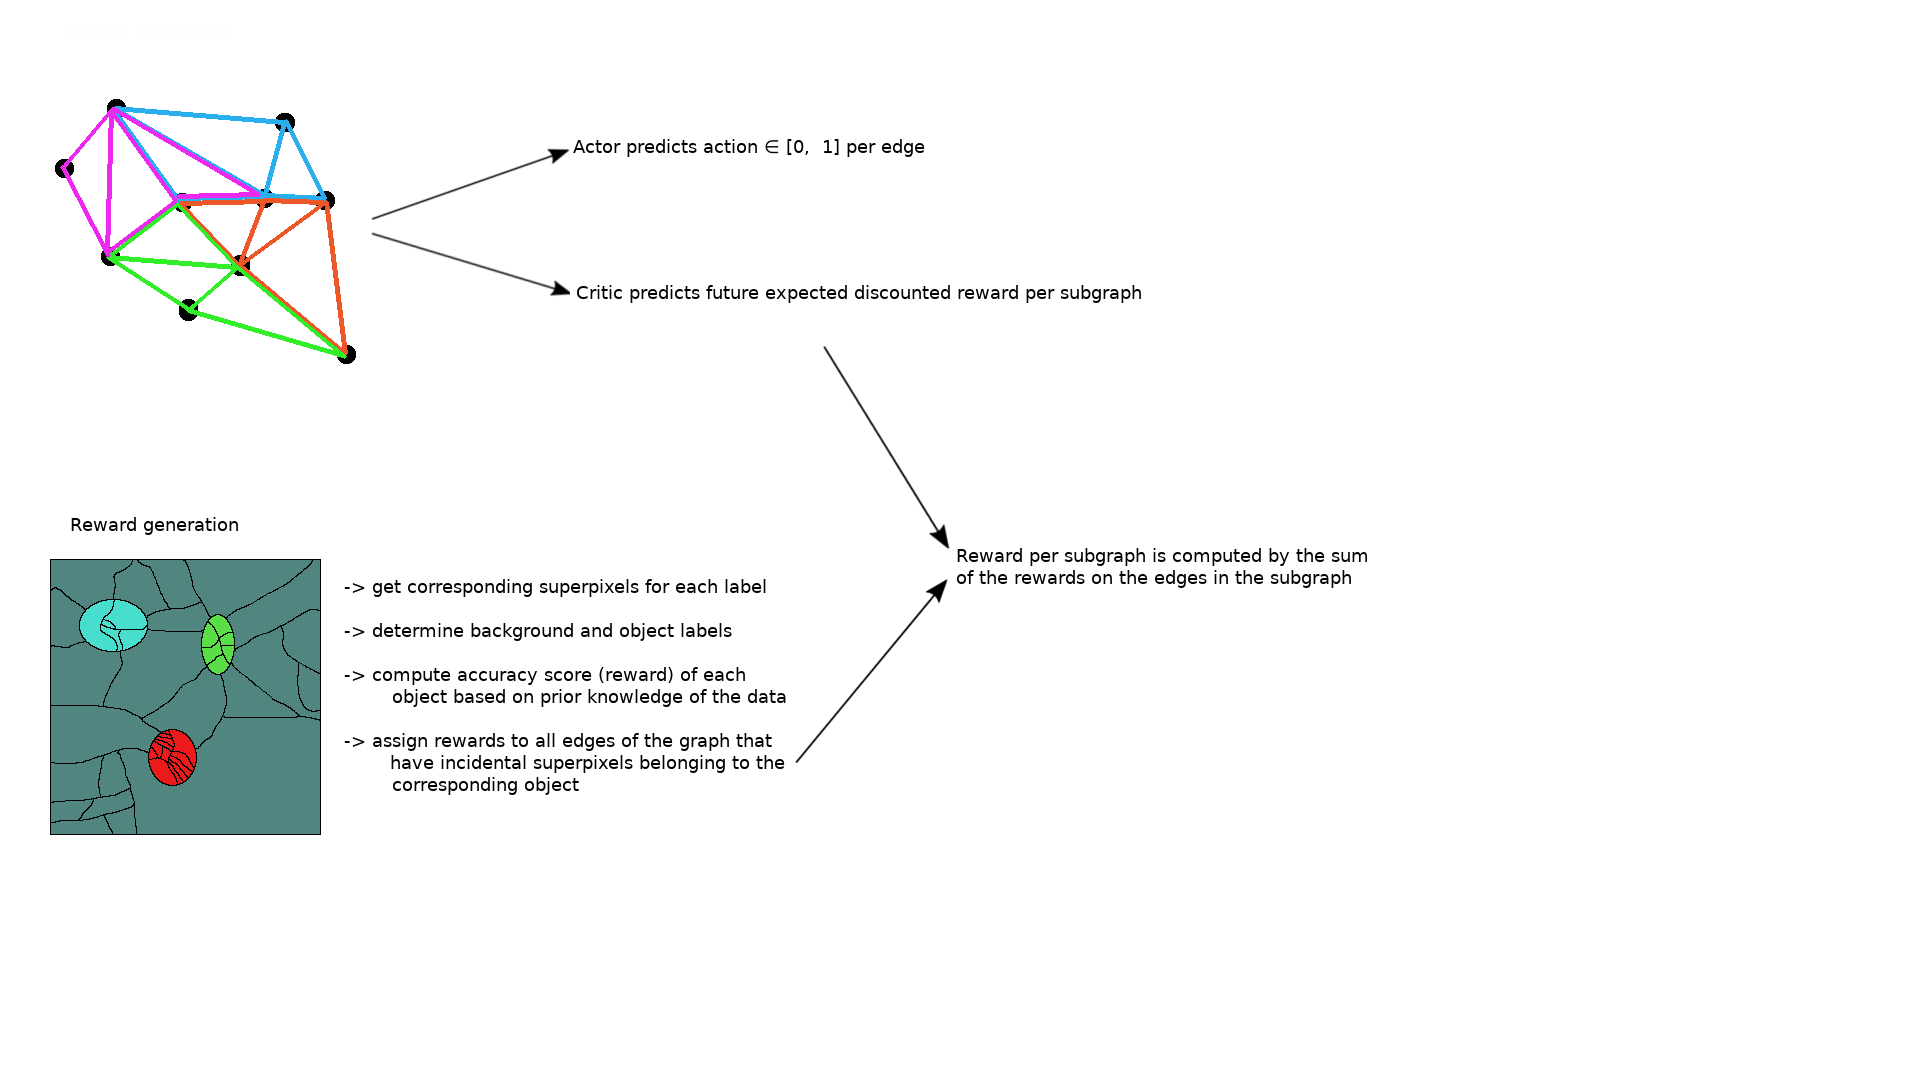
\includegraphics[width=1.5\textwidth]{figures/images/reward_calc_sketch.png}
	\caption{A rough sketch of the reward calcuation on subgraphs with 7 edges and the resulting losses in an actor critic setting}
	\label{reward_calc}
\end{figure}

\subsection{Definition of the RL algorithm}
Most RL algorithms like Q-learning operate in discrete action spaces. The advantages of that have been mentioned. However for the prediction of probabilities it is more natural to use a continuous action space. The drawback is that it is possible to diverge fast from an initial state. Such a divergence can easily be penalized by the reward signal e.g by calculating the distance of current state to the initial state and subtracting that distance from the reward when it surpasses a certain margin. \\
Therefore the SAC algorithm \ref{ssec:sac} is used which is a comfortable choice because it is defined for continuous actions and, by construction, it takes care of sufficient exploration. 

It is easy to adjust eq. (2.26) in section \ref{ssec:sac} for predictions on subgraphs. Considering a subgraph size of $10$ and selecting the Normal distribution for the policy $\pi$. A policy GCNN predicts for every edge mean $\mu$ and variance $\sigma ^2$ of its respective action distribution. \\
Drawing a reparameterized \ref{ssec:reparam} sample from this distribution follows a Sigmoid transform of the sample. Since the Sigmoid function is a diffeomorphism, the change of variables formula \cite{papamakarios2019normalizing} can be applied and allows for the computation of the probability density of the transformed sample. \\
The joint probability density of all actions per subgraph is given by the product of their respective densities. Therefore eq. (2.26) in section \ref{ssec:sac} is rewritten as

\begin{align}
	\nabla_\theta \bar{\mathcal{L}}_{actor} = \nabla_\theta \sum_{sg \in G} \left[ \alpha \sum_{a_t\in sg}log(\pi(a_t|s_t)) - Q_\pi(s_t, a_t)_{sg} \right]
\end{align}

Here $G$ is the set of sets that contain the respective actions for each subgraph. $Q_\pi(s_t, a_t)$ is a function mapping the current state action tuple $(s_t, a_t)$ to $\mathbb{R}^n$ where $n$ is the number of subgraphs in $s_t$. $Q_\pi(s_t, a_t)_{sg}$ denotes the predicted state action value for subgraph $sg$.\\
Eq. (2.22) in section \ref{ssec:sac} does not change considering the rewards are per subgraph as well.\\
Additionally to the optimization techniques within the SAC \ref{ssec:sac} algorithm, prioritized experience replay \ref{ssec:common_opt} is used.\\
RL problems are usually of the form that, starting from an initial state $s_0$, multiple steps lead to an end state $s_T$. Since here, directly sampling affinity values from the policy makes it possible to reach any state within one step, it is sufficient to define $T=1$. Stopping after one step has the advantage that the state action function becomes much simpler. The feature to be able to reach any state from any other state makes all parts of the state that are dependent on $t$ redundant. Therefore $s_t$ can be redefined to $s_t=s=[rw, sp]$. Setting $T=1$ the loss in eq. (2.22) in section \ref{ssec:sac} becomes

\begin{align}
	\mathcal{L}_{critic} = \frac{1}{2}(Q_{\pi}(s_t, a_t) - r_t) ^ 2
\end{align}

While this yields a simple action state function to approximate, there is also a point in saying that this definition is not a "real" RL setting anymore. However the RL loss still gives the advantage that the supervision signal (here the reward), does not have to be differentiable, which is the main justification for this pipeline.